\documentclass[12pt]{article}
\usepackage{fontspec}
\usepackage{xunicode}
\usepackage{polyglossia}
\setmainlanguage{french}
\usepackage{csquotes}

\usepackage{soul}
\usepackage{color}

\usepackage{enumitem}
\usepackage{setspace}

\usepackage{lscape}
\usepackage{graphicx}
\usepackage{float}

\title{Cahier des charges - Application sur les résultats des pays aux Jeux Olympiques}
\date{}
\author{T. Burnel, N. Grim, M. Griveau, M. Mechentel}

\begin{document}
	\setstretch{1.5}
	\maketitle
	\tableofcontents
	
	\section{Introduction}
	
	Notre projet est de créer une application web permettant de consulter les résultats de différents pays à diverses éditions des Jeux Olympiques.
	
	Les utilisateurs pourront sélectionner le pays de leur choix et constater le nombre de médailles d'or, d'argent et de bronze remportées par sport -- le tout en fonction des investissements dans le domaine sportifs du pays sélectionné.
	
	\section{Données}
	
	\subsection{Jeux de données}
	
	Nos jeux de données sont les suivants :
	
	\begin{itemize}
		\item Un jeu de données issu de la plateforme Kaggle, présentant le nombre de médailles remportées par sport et par athlète sur 120 ans ;
		\item Un jeu de données issu du FMI présentant les investissements dans le domaine du sport par pays sur une période d’une trentaine d’années.
	\end{itemize}

	\subsection{Modèle de données}
	
	Nous avons choisi de représenter nos données au sein d'une base relationnelle dont voici la représentation :
	
	\begin{center}
		\begin{figure}[H]
			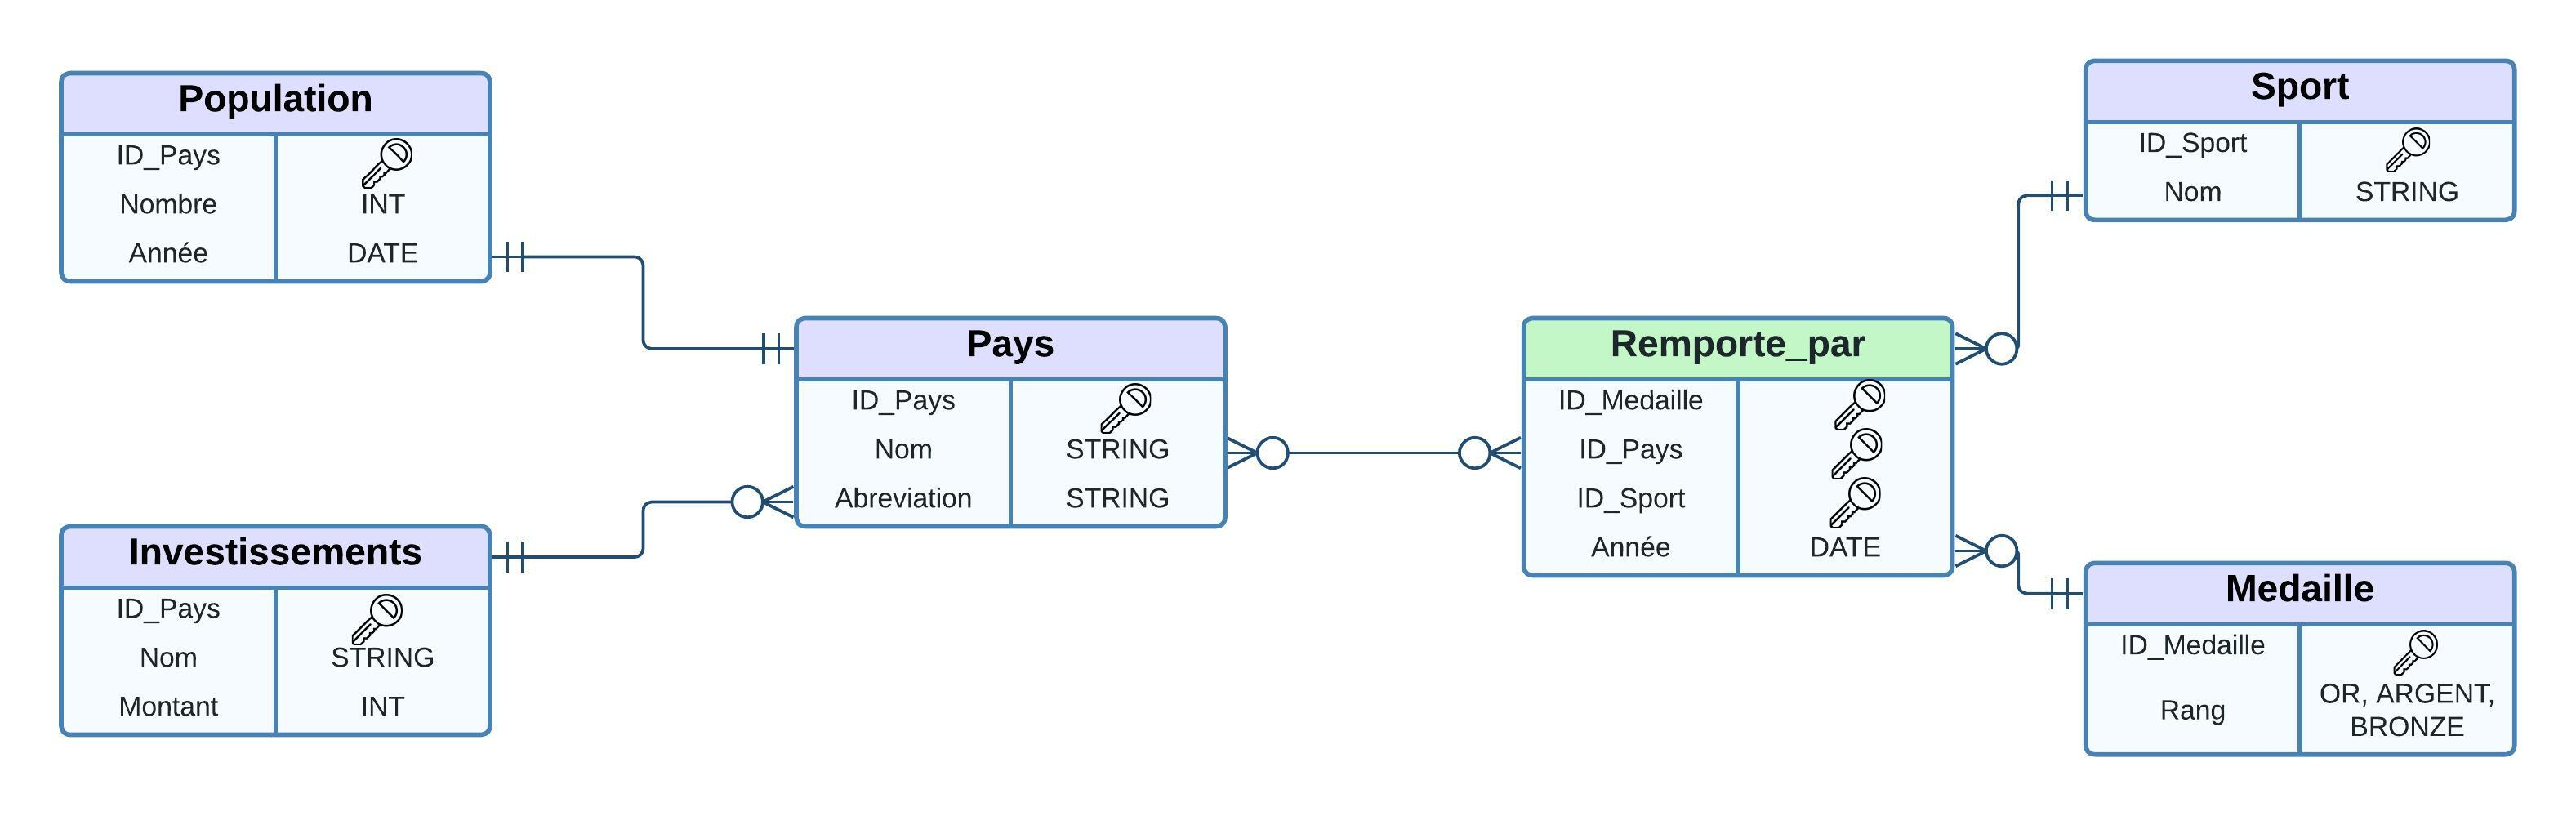
\includegraphics[scale=0.5]{modele01.jpeg}
		\end{figure}
	\end{center}

	\section{Routes}
	
	Nous avons songé aux routes suivantes :
	
	\begin{itemize}
		\item Une route redirigeant vers une page d'accueil :
		\begin{itemize}
			\item \textbf{localhost:5000/accueil}
		\end{itemize}
		\item Une route visualisation avec une carte du monde, permettant de sélectionner un pays en particulier :
		\begin{itemize}
			\item \textbf{localhost:5000/visualisation}
		\end{itemize}
		\item Une route permettant de visualiser les résultats du pays sélectionné :
		\begin{itemize}
			\item \textbf{localhost:5000/visualisation/<uuid>}
		\end{itemize}
		\item Une route de fonctionnalité souhaitée permettant d'accéder à sa bibliothèque de rubriques :
		\begin{itemize}
			\item \textbf{localhost:5000/rubriques}
		\end{itemize}
	\end{itemize}

	\section{Fonctionnalités}
	
	\subsection{Fonctionnalités requises}
	
	\begin{itemize}
		\item Gestion des utilisateurs :
		\begin{itemize}
			\item Inscription, connexion, déconnexion ;
		\end{itemize}
		\item Gestion du profil :
		\begin{itemize}
			\item Nom d'utilisateur, mail, mot de passe ;
		\end{itemize}
		\item Ajout de certains sports/pays en favori :
		\begin{itemize}
			\item Ces informations pourraient être stockées dans une base de données. L'utilisateur pourra les modifier et les supprimer.
		\end{itemize}
	\end{itemize}

	\subsection{Fonctionnalités souhaitées}
	
	\begin{itemize}
		\item Changement du mot de passe :
		\begin{itemize}
			\item envoi d'un formulaire temporaire par mail pour réinitialiser le mot de passe ;
		\end{itemize}
		\item Réception de notifications :
		\begin{itemize}
			\item Soit chaque fois qu'une médaille est remportée (peu importe le sport, le rang et le pays) ;
			\item Soit selon les favoris de l'utilisateur ;
		\end{itemize}
		\item Création de collections :
		\begin{itemize}
			\item Création de collections personnalisées (par exemple : \enquote{Sports collectifs}, \enquote{Pays d'Europe}, etc.)
		\end{itemize}
	\end{itemize}
	
	\section{Étapes du développement}
	
	\subsection*{Instanciation du modèle de données}
	
	Charge de travail : une personne, une semaine.
	
	\subsection*{Gestion des utilisateurs}
	
	Charge de travail : deux personnes, deux semaines.
	
	\subsection*{Structuration des templates avec Jinja}
	
	Charge de travail : deux personnes (une pour les templates HTML/CSS, une pour Jinja et les routes), deux semaines.
	
	\subsection*{Visualisation des données}
	
	Charge de travail : une personne, deux semaines.
	
	\subsection*{Interaction avec les données}
	
	Charge de travail : une personne, deux semaines.
		
\end{document}
